\documentclass{article}

\usepackage[utf8]{inputenc}
\usepackage[german]{babel}
\usepackage{amsmath}
\usepackage{mathtools}
\usepackage{listings}
\usepackage{color}

\lstset{
  language=C,
  numbers=left,
  stepnumber=1,
  numbersep=5pt,
  backgroundcolor=\color[rgb]{0.9,0.9,0.9},
  showspaces=false,
  showstringspaces=false,
  showtabs=false,
  tabsize=2,
  captionpos=b,
  breaklines=true,
  breakatwhitespace=true,
  title=\lstname,
}

\begin{document}

\tableofcontents

\section{Betriebssystem}

\subsection{Definition}

\begin{itemize}
    \item \textbf{Systemsicht} \\
        Alle Programme zur \textbf{Steuerung und Überwachung} von:
        \begin{itemize}
            \item Ausführung v. Benutzerprogrammen
            \item Verteilung der Betriebsmittel
            \item Aufrechterhaltung der Betriebsart
        \end{itemize}
    \item \textbf{Anwendersicht} \\
        \textbf{Virtuelle Maschine}, vereinfachte Ansicht des Computers
\end{itemize}

\subsection{Aufgaben}

\begin{itemize}
    \item \textbf{Hardwareabstraktion}
    \begin{itemize}
        \item einheitliche Sicht auf Geräteklassen
        \item Bibliotheken und Treiber
    \end{itemize}

    \item \textbf{Resourcenverwaltung}
    \begin{itemize}
        \item CPU-Rechenzeit
        \item Speicher
        \item Gerätezugriffe
    \end{itemize}

    \item \textbf{Sicherheitsfeatures}
    \begin{itemize}
        \item Benutzer und Gruppen \textbf{Multi-User}
        \item Parallelbetrieb \textbf{Multitasking}
        \item Schutz for direkten Hardwarezugriffen
    \end{itemize}
\end{itemize}

\subsection{Arten}
\begin{itemize}
    \item \textbf{Mainframe}
        schnelles I/O, viele Prozesse, Transaktionen
    \item \textbf{Server}
        viele Anwender, Netzanbindung    
    \item \textbf{Multiprozessor}
    \item \textbf{Echtzeit}
\end{itemize}
\section{Prozesse}

\subsection{Bestandteile}
\begin{itemize}
    \item eigener Adressraum
    \item Programmcode
    \item Programmdaten
    \item Programm-Counter
    \item Stacks und Stackpointer
    \item Hardwareregister-Inhalte \textit{(Prozess-Kontext)}
    \item Heap-Speicher
    \item Verwaltungsdaten
    \begin{itemize}
        \item Identifier und VaterID
        \item Resourcenliste
        \item Scheduling Parameter
    \end{itemize}
\end{itemize}

\begin{figure}[ht!]
    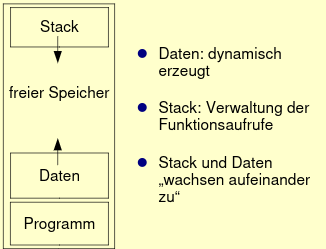
\includegraphics[scale=.75]{pics/processes}
    \caption{Process Control Block PCB}
\end{figure}

\subsection{Hierarchie und Signale}
Jeder Prozess hat \textbf{Vaterprozess} \textit{(Prozesse erzeugen einander)}.

\subsubsection{Fork}
\begin{lstlisting}
    int pid = fork();
    if(pid == 0){
        printf("Ich bin das Kind mit pid=%d\n", getpid());
    }else if(pid > 0){
        printf("Ich bin der Vater, mein Kind hat die pid=%d\n", pid);
    }else{
        printf("Error: fork() war nicht erfolgreich");
    }
\end{lstlisting}

\subsubsection{Signale}
\begin{itemize}
    \item (17) STOP \textit{(Strg-Z oder bg)}
    \item (19) CONT \textit{(fg)}
    \item (15) SIGTERM \textit{(beenden)}
    \item (9) KILL \textit{(abschließen)}
\end{itemize}

\subsection{Prozesserzeugung}
\begin{enumerate}
    \item fork $\rightarrow$ clone $\rightarrow$ do\_fork $\rightarrow$ copy\_process
    \item neue thread\_info in task\_struct
    \item Kind-Status auf TASK\_UNINTERRUPTABLE
    \item copy\_flags
    \item get\_pid: neue PID für Kind
    \item je nach clone-Parametern: kopieren/gemeinsam nutzen
    \item Scheduler
\end{enumerate}
\section{Threads}
\begin{itemize}
    \item Aktivitätsstrang in einem Prozess
    \item gemeinsamer Zugriff auf Daten
\end{itemize}

\subsection{Vergleich: Prozesse/Threads}

\subsubsection{Gemeinsam mit Prozess:}
\begin{itemize}
    \item Adressraum
    \item Programmcode
    \item aktuelle Daten (Variablen/Konstanten)
\end{itemize}

\subsubsection{Separat pro Thread}
\begin{itemize}
    \item PC
    \item SP
    \item Stack
    \item Register
\end{itemize}

\begin{figure}[ht!]
    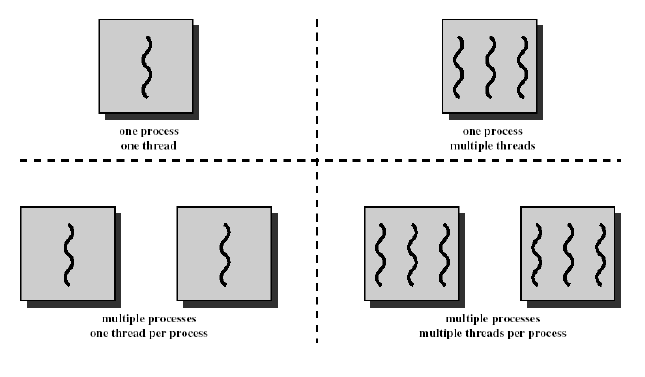
\includegraphics[width=\linewidth]{pics/processes_vs_threads}
    \caption{Unterschied zw. Prozessen und Threads}
\end{figure}

\subsection{User - und Kernel-Level Threads}

\subsubsection{User-Level Threads}
\begin{itemize}
    \item Keine Systemcalls nötig
    \item Blockiert bei I/O
    \item keine Nutzung mehrerer CPUs
    \item Bessere Abstraktion möglich
\end{itemize}

\subsubsection{Kernel-Level Threads}
\begin{itemize}
    \item BS verwalted Threads
    \item Zeitsteuerung nur mit Systemcalls
\end{itemize}

\subsubsection{Kombinierte Threadtypen}
\begin{figure}[ht!]
    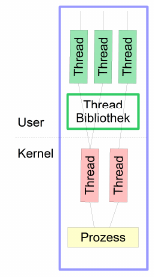
\includegraphics[scale=.8]{pics/ultklt}
    \caption{Komtiniert: ULT, KLT}
\end{figure}

\subsection{Linux Threads und Prozesse}
\textbf{Prozesse} und \textbf{Threads} werden in Linux einheitlich gehandhabt:
\begin{lstlisting}
    // Prozess
    clone(SIGCHLD, 0);
    // Thread
    clone(CLONE_VM | CLONE_FS | CLONE_FILES | CLONE_SIGHAND, 0);
\end{lstlisting}

\begin{figure}[ht!]
    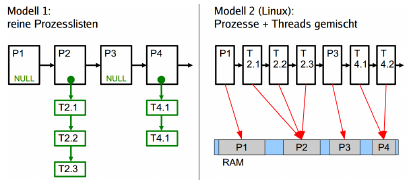
\includegraphics[scale=.8]{pics/linux_ps_th}
    \caption{Linux Prozess- und Threadverwaltung}
\end{figure}

\section{Interrupts}
\subsection{Interrupt-Klassen}
\begin{itemize}
    \item Hardware-Fehler
    \item Timer
    \item I/O
    \item Software-Interrupts
    \begin{itemize}
        \item Arithmetik
        \item Traps
        \item etc.
    \end{itemize}
\end{itemize}

\subsection{Ablauf}
\begin{enumerate}
    \item Interrupt flag wird gesetzt
	\item Nach aktuellem Befehl wird unterbrochen (BS übernimmt Kontrolle)
	\item Prozess-Daten werden gespeichert (wie bei Kontextswitch)
	\item Mittels Interrupt-Vector wird die entsprechende ISR aufgerufen
	\item Diese ist nicht unterbrechbar und so kurz wie möglich
	\item Die ISR ruft dann ein sog. Tasklet auf welches unterbrechbar ist und die eigentliche Arbeit macht
\end{enumerate}

\subsection{Round Robin: I/O- vs CPU-lastig}
\textbf{CPU-lastinge} Prozesse nutzen ihre \textbf{Zeitquanten} vollständig, während \textbf{I/O}
Prozesse \textbf{warten} müssen.

\subsection{Interrupt Handling}
\begin{figure}[ht!]
    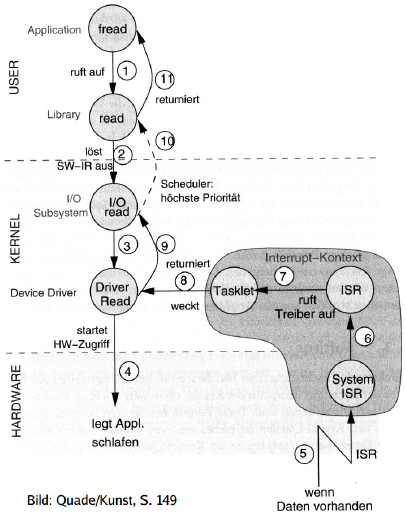
\includegraphics[scale=.8]{pics/isr}
    \caption{Interrupt callgraph}
\end{figure}
\section{Scheduling}

Scheduling: Zuteilug der CPU (Betriebsmittel) an Threads/Prozesse

\subsection{Wann wird der Scheduler aktiv}
\begin{itemize}
    \item neuer Prozess entsteht
    \item aktiver Prozess endet
    \item Prozess wg. I/O blockiert
    \item Zeitquantum is aufgebraucht
    \item Interrupt tritt auf
\end{itemize}

\subsection{Scheduling-Prinzipien}
\begin{itemize}
    \item Kooperativ
    \item Präemptiv
    \item Batch
    \begin{itemize}
        \item FCFS
        \item SJF
        \item SRF
        \item Prioritäten
    \end{itemize}
\end{itemize}

\subsection{Kriterien}

\subsubsection{Anwendersicht}
\begin{itemize}
    \item Ausführungsdauer (Prozess-Gesamtlaufzeit)
    \item Reaktionszeit (Reaktionen auf Benutzerinteraktionen)
    \item Deadlines
    \item Vorhersagbarkeit (gleichartige Prozesse)
    \item Proportionalität
\end{itemize}

\subsubsection{Systemsicht}
\begin{itemize}
    \item Durchsatz (Prozesse pro Zeit)
    \item Prozessauslastung (Cycles pro Zeit)
    \item Fairness (keine starvation)
    \item Prioritäten
    \item Resourcen Fairness
\end{itemize}

\subsection{Round Robin und I/O}
\subsubsection{Virtual Round Robin}
\begin{figure}[ht!]
    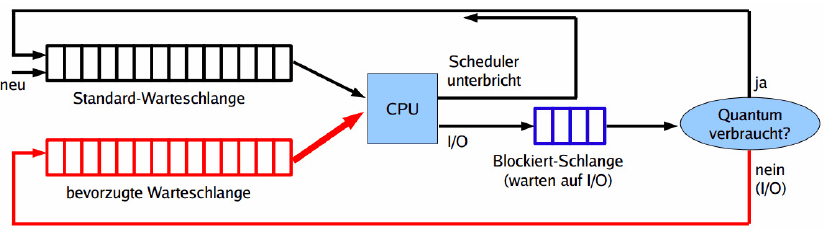
\includegraphics[scale=.4]{pics/virtual_round_robin}
    \caption{Virtual round robin prinzip}
\end{figure}

\subsubsection{Prioritätsbasiert}
\begin{itemize}
    \item Dynamisch (+ variable Quantenlänge): z.B. Aging (~SJF)
    \item Multilevel Scheduling
\end{itemize}

\textbf{Priority-Inversion:}
\begin{figure}[ht!]
    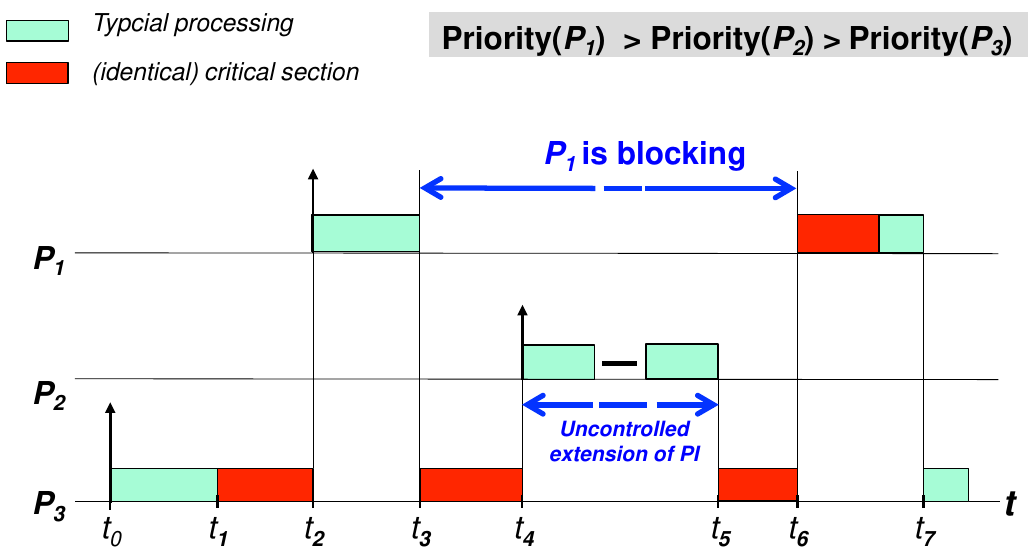
\includegraphics[scale=.3]{pics/priority_inversion}
    \caption{Beispiel für Priority-Inversion}
\end{figure}

\subsection{Formeln}
\subsubsection{Burstdauer}
\begin{itemize}
    \item $S_{n+1} = \frac{1}{n} \sum_{i=1}^n T_i = \frac{1}{n} T_n + \frac{n-1}{n} S_n$
    \item $S_{n+1} = \alpha T_n + (1-\alpha) S_n; \alpha \in [0,1]$
\end{itemize}
\section{Synchronisation}

\subsection{Race Condition}
mehrere parallele Threads/Prozesse nutzen \textbf{gemeinsame Resource}.\\
Zustand hängt von Ausführung ab:\\
$\Rightarrow$ \textbf{nicht vorhersagbar, nicht reproduzierbar}

\subsection{Synchronisationsmechanismen}
\begin{itemize}
    \item Mutex
    \item Semaphor
    \item Event(-Queue)
    \item Monitor
    \item Locking
\end{itemize}

\subsection{Anforderungen}
\begin{itemize}
    \item kein Deadlock (blockiert außerhalb v. kritischem Bereich)
    \item Starvation free (Scheduling bei mehreren Wartenden)
\end{itemize}
\section{Interprozesskommunikation IPC}

\subsection{Charakteristika}
\begin{itemize}
    \item Kommunikationsmodell
    \begin{itemize}
        \item P2P
        \item publish-subscribe
        \item broadcast
    \end{itemize}
    \item Übertragungsrichtung
    \begin{itemize}
        \item simblex
        \item duplex
    \end{itemize}
    \item Synchronität
    \begin{itemize}
        \item synchron/blockierend
        \item asynchron/nicht-blockierend (nachrichtenbasiert)
    \end{itemize}
\end{itemize}

\subsection{Basismechanismen (Linux)}
\begin{itemize}
    \item Signale
    \item Synchronisation (prozessübergreifend)
    \begin{itemize}
        \item shared mutex
        \item shared semaphore
    \end{itemize}
    \item Pipes (unix)
    \begin{itemize}
        \item FIFO Bytestream
        \item unidirektional
        \item Synchron
    \end{itemize}
    \item Sockets
    \begin{itemize}
        \item Verbindungslos UDP
        \item Verbindungsorientiert TCP
    \end{itemize}
    \item Shared-Memory
\end{itemize}

\subsection{Middleware-Lösungen}
\begin{itemize}
    \item Synchron
    \begin{itemize}
        \item RPC
        \item RMI (Java)
        \item CORBA
        \item DBus Messaging (~RPC)
    \end{itemize}
    \item Asynchron
    \begin{itemize}
        \item SmartSockets
        \item MqSeries Messaging
        \item JMS
    \end{itemize}
\end{itemize}

\section{Speicherverwaltung}
\begin{figure}[ht!]
    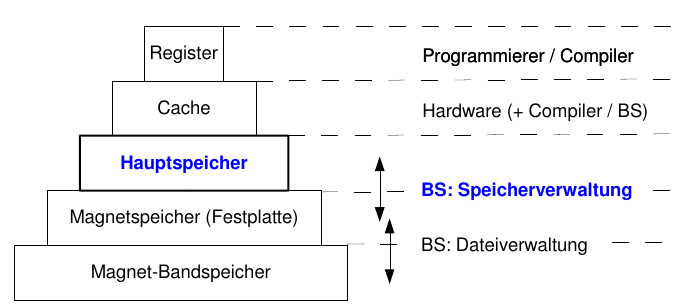
\includegraphics[scale=.5]{pics/memory}
    \caption{Speicherhierarchie}
\end{figure}

\subsection{Aufgaben}
\begin{itemize}
    \item Finden und Zuteilung freier Speicherbereiche
    \item Effiziente Nutzung des Speichers
    \item Speicherschutz
\end{itemize}

\subsection{Code-Verschiebung (Relokation)}
\begin{enumerate}
    \item Linker vermerkt absolute Adressen, werden beim Laden abgeändert
    \item oder: bei jeder Adressberechnung wird ein Basisregister hinzuaddiert
\end{enumerate}

\pagebreak

\subsection{Speicherschutz}
\begin{figure}[ht!]
    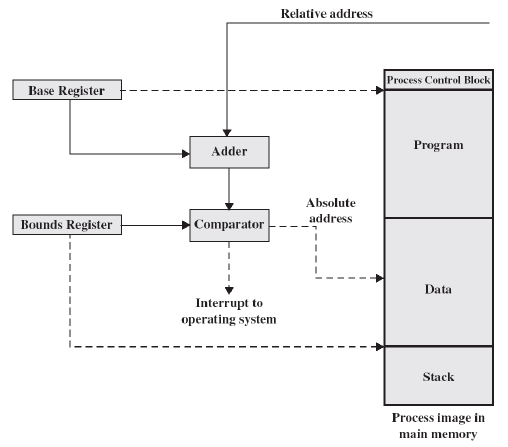
\includegraphics[scale=.6]{pics/memory_access}
    \caption{Speicherschutz}
\end{figure}

\subsection{Zusammenhängende Speicheraufteilung}
Aufteilung des Speichers in Partitionen fester größe

\begin{itemize}
    \item Fragmentierung (kleine Bereiche im Speicher sind ungenutzt)
    \item Relokation (Speicherbereiche werden verschoben)
    \item Swapping (Speicherbereiche werden auf die Festplatte verschoben)
\end{itemize}

\subsubsection{Suchverfahren für freien Speicher}
\begin{itemize}
    \item First Fit
    \item Worst Fit
    \item Best Fit
    \item Quick Fit (mehrere Listen mit verschiedenen Bereichsgrößen) (Buddy System)
\end{itemize}

\subsection{Nicht Zusammenhängende Speicheraufteilung}
Memory Management Unit (MMU) bildet jede logische Adresse auf eine Physische ab.

\subsubsection{Paging}
Aufteilung der Adressräume in Blöcke fester Größe.
\begin{itemize}
    \item Page: Block im virtuellen Adressraum
    \item page frame: Block im physischen Adressraum
\end{itemize}

\begin{figure}[ht!]
    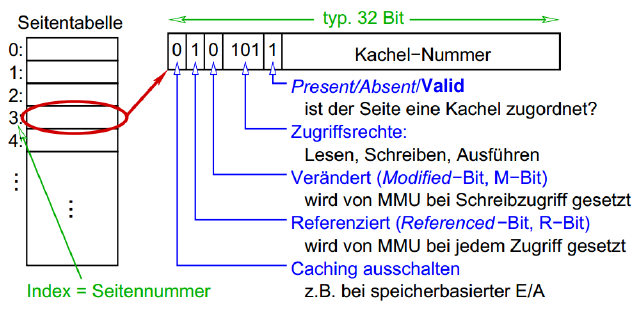
\includegraphics[scale=.5]{pics/pagetable}
    \caption{Seitentabelle}
\end{figure}

\pagebreak


\subsubsection{Translation Look-Aside Buffer}
\begin{itemize}
    \item Durch das Lokalitätsprinzip, kann der TLB hohe Trefferquoten erzielen.
    \item Bei Prozesswechesl
    \begin{itemize}
        \item valid bit für alles gelöscht
        \item jeder Eintrag hat PID
    \end{itemize}
\end{itemize}

\begin{figure}[ht!]
    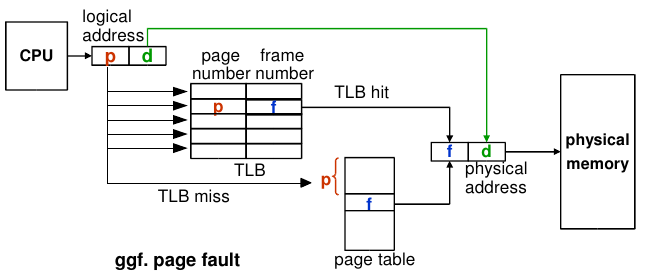
\includegraphics[scale=.5]{pics/tlb}
    \caption{Translation Lookaside Buffer}
\end{figure}

\subsubsection{Aufbaben: Betriebssystem und Hardware}

\textbf{Betriebssystem:}
\begin{itemize}
    \item Page-Table-Register Laden
    \item Page fault behandeln
    \item Seitenverdrängung
\end{itemize}

\noindent\textbf{Hardware}
\begin{itemize}
    \item Zugriff auf TLB
    \item Adressumrechnung
\end{itemize}

\subsubsection{Mehrstufiges Paging}
z.B. 32-Bit Adressen p1(10), p2(10), p3(12)

\pagebreak

\subsubsection{Pagefaults}
\begin{figure}[ht!]
    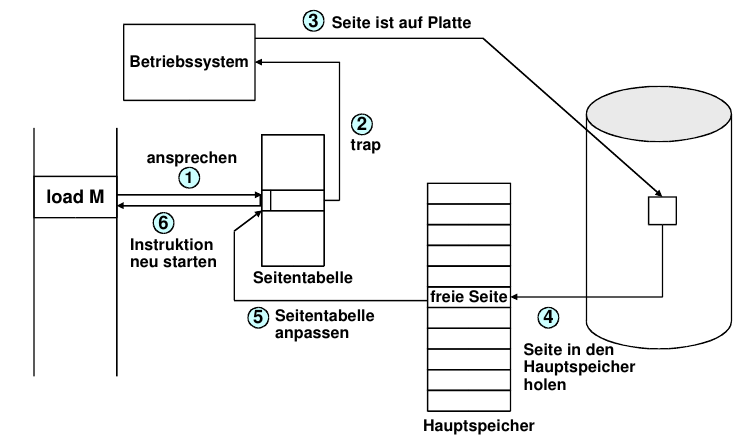
\includegraphics[scale=.4]{pics/pagefault}
    \caption{Pagefault Behandlung}
\end{figure}

\subsubsection{Verdrängungsstrategie}
\begin{itemize}
    \item Not Recently Used (referenced bit \textit{(regelmäßiger reset)} und modified bit)
    \begin{itemize}
        \item 0: nicht referenziert, nicht modifiziert
        \item 1: nicht referenziert, modifiziert
        \item 2: referenziert, nicht modifiziert
        \item 3: referenziert, modifiziert
    \end{itemize}
    \item Second-Chance
    \begin{figure}[ht!]
        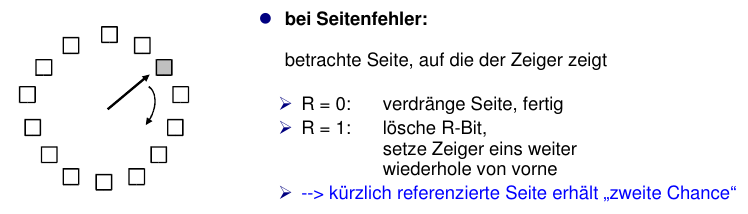
\includegraphics[scale=.3]{pics/second_chance}
        \caption{Second-Chance Algorithmus}
    \end{figure}
    \item Least Recently Used (Umsetzung des Zeitstempels ist problematisch)
\end{itemize}

\subsubsection{Trashing}
Entsteht wenn mehr Seiten aktiv sind als Seitenrahmen verfügbar.\\\\

\textbf{Abrufstrategien}
\begin{itemize}
    \item Demandpaging (erst bei Bedarf)
    \item Prepaging (z.B. bei Programmstart)
    \item asynchron (wenn gerade wenig last)
    \item Clustering (bei Fault ganzes cluster)
    \item Locking (Ausnahmen beim Paging)
\end{itemize}


Mittlere Speicherzugriffszeit bei Warscheinlichkeit \textbf{p} für Seitenfehler:
\begin{equation*}
    t_z = t_{HS} + p \cdot t_{PF}
\end{equation*}
\begin{itemize}
    \item $t_{HS}$: Zugriffszeit auf Hauptspeicher
    \item $t_{PF}$: Zeit für Behandlung
    \item \textit{(p sollte klein sein: sonst trashing)}
\end{itemize}


\end{document}
